\chapter{Grafická časť aplikácie (frontend)}
V rámci frontend časti aplikácie boli použité aplikácie:\begin{itemize}
\item \textbf{QT4 designer} - softvér na návrh dizajnu okien aplikácie
\item \textbf{PyQT 4} - doplnok do pythonu, na návrh a programovanie grafických aplikácií
\end{itemize} 
\section{QT4 disigner}
QT4 designer je aplikácia na návrh šablón v rámci použitia knižnice PyQT4. Designer patrí k štandardným nástrojom PyQt knižnice a nachádza sa v \textit{/usr/lib/x86\_ 64-linux-gnu/qt5/bin/designer}. Medzi základné objekty použité v aplikácii sem patria:
\begin{itemize}
\item \textbf{QPushButton} - tlačítko v GUI
\item \textbf{textlabel} - popis pri tlačítkach a textových poliach
\item \textbf{textedit} - pole na text, obsahuje metódy napr. \textit{text()}
\item \textbf{QListWidget} - časté použitie v aplikácii, napr. pri použití zobrazenia prvkov po stalčení tlačítka, správa prvkov v objekte,objekt je klikateľný, editovateľný, ...
\item \textbf{lineedit} - textové pole na editáciu riadku
\end{itemize} 
Po vytvorení šablóny sa súbor uloží vo formáte \textit{.ui} a musí sa nahrať do kódu aby sa s ním dalo pracovať pomocou príkazu \textit{qtCreatorFile = "súbor.ui"}
\section{PyQT 4}
V aplikácii je použitá verzia PyQT vo verzii 4. Dnes existuje v dvoch verziách a to vo verzii 4 a vo verzii 5. Nakoľko QT4 designer je navrhnutý na PyQT vo verzii 4, tak aj PyQT je v kóde použité vo verzii 4. \\
V rámci okna po prihlásení na zariadenie je okno založené na objekte \textit{menubar()} a na metódach \textit{addMenu()} na pridávanie hlavných položiek v menu a ďalšie položky sú \textit{QAcion}, ktoré vytvárajú podzložku v menu cez metódu \textit{addAction()}. Ďalšou dôležitou knižnicou je \textit{QtGui} na vytvorenie GUI plikácie. Objekt \textit{QApplication()} vytvorí samostatnú aplikáciu spoločne s metódou pre otvorenie okna \textit{show()}, tiež je tu použitá knižnica \textit{sys} a jej metóda \textit{exit()} na zatvorenie celej aplikácie,  a ďalšou metódou je \textit{close()}, táto metóda okno zavre.
\chapter{Grafická aplikácia}
\section{Hlavné prihlasovacie okno}
Hlavné okno aplikácie predstavuje prihlasovaciu obrazovku a možnosť zobrazenia blízkych zariadení a to ich IP adries pomocou tlačítka \textit{find devices}(vyhľadávacia doba je 2x 30 sekúnd, najskôr vyhľadá MAC adresy, potom IP adresy), pomocou tohoto tlačítka sa vylistujú blízke mikrotik zariadenia a ich IP adresy, toto vychádza z aplikácie mactelnet a výstup zachytáva \textit{listIpValues a listMacValues}. Toto vidíme na obrázku \ref{fig:winboxlinux}.
\begin{figure}[H]
\centering
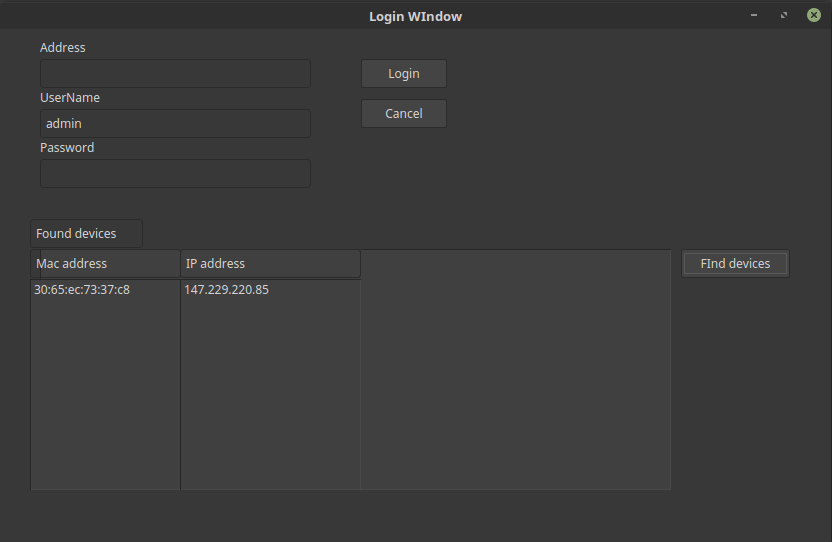
\includegraphics[scale=0.45]{../text/winboxnew.png}
\caption{Prihlasovacie okno aplikácie}
\label{fig:winboxlinux}
\end{figure}
Ďalej sa tu nachádzajú textové polia address, username a password. Do týchto polí sa zapisuje IP adresa (je možné ju skopírovať z IP address textového poľa) zariadenia, na ktoré sa chceme pripojiť, užívateľské meno  a heslo a po stlačení tlačítka \textit{login} sa užívateľ pri úspešnom pokuse prihlási na mikrotik pomocou \textit{API-SSL}. V opačnom prípade sa vyhodí okno s výnimkou. Pri nepodpore zariadenia API-SSL prípadne španej komunikácie v rámci overovania certifikátu sa vyhodí nasledujúca výnimka podľa obrázku \ref{fig:socket}. Druhým typom výnimky je neúšpešné prihlásenie chybného užívateľského mena alebo hesla. Toto vidíme na obrázku \ref{fig:loginworong}.Všetky tieto výnimky sú spravované pod štandardnými výnimkami programovacieho jazyka python a používajú štandardne \textit{try except}.
\begin{figure}[h!]
\centering
\begin{subfigure}{.6\textwidth}
  \centering
  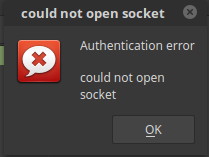
\includegraphics[width=.5\linewidth]{../text/socket.png}
  \caption{Výnimka pri zlej komunikácii s routrom}
  \label{fig:socket}
\end{subfigure}%
\begin{subfigure}{.6\textwidth}
  \centering
  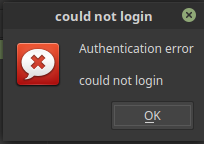
\includegraphics[width=.5\linewidth]{../text/loginerror.png}
  \caption{Výnimka pri zlom prihlásení}
  \label{fig:loginworong}
\end{subfigure}
\caption{Zoznam výnimiek pri prihlásení na zariadenie}
\label{fig:exceptions}
\end{figure}
%\begin{figure}[H]
%\centering
%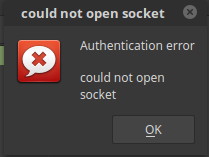
\includegraphics[scale=0.55]{../text/socket.png}
%\caption{Výnimka pri španej komunikácii s routrom}
%\label{fig:socket}
%\end{figure}
%\begin{figure}[H]
%\centering
%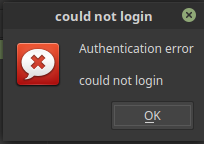
\includegraphics[scale=0.55]{../text/loginerror.png}
%\caption{Výnimka pri zadaní zlého užívateľského mena alebo hesla}
%\label{fig:loginworong}
%\end{figure}
\subsection{Hlavné okno konfiguračnej aplikácie}
Po úspšnom prihlásení na zariadení sa otvorí okno popisujúce na obrázku \ref{fig:loginokno}.
\begin{figure}[H]
\centering
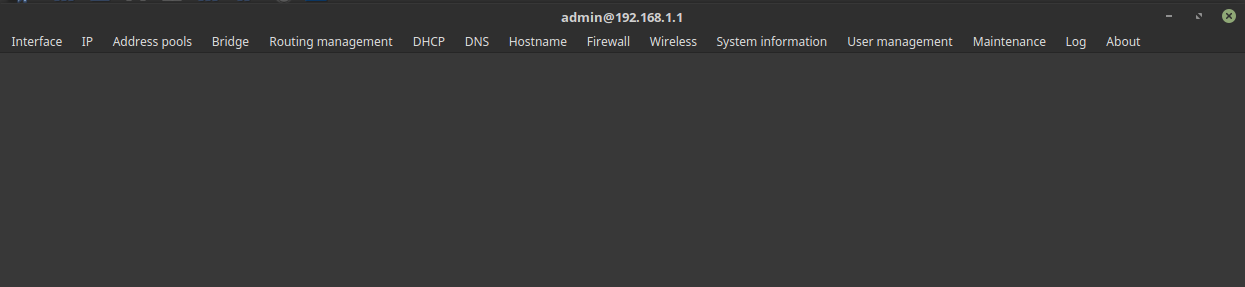
\includegraphics[scale=0.35]{../text/loginokno.png}
\caption{Hlavné okno aplikácie}
\label{fig:loginokno}
\end{figure}
Aplikácia je riešená podobne ako na mikrotiku, to znamená okno v okne. Aplikácia je viac-oknová, može sa otvoriť niekoľko okien naraz a okná budú vykreslené v hlavnom okne aplikácie. 
\section{Položky hlavného menu}
\label{sec:buttons}
V menu sa nachádzajú jednotlivé položky a ich podzložky:
\begin{itemize}
\item \textbf{Interface} - správa a manažment rozhraní, pridávanie, odoberanie rozhraní, zapnutie a vypnutie rozhraní, obshauje tiež správu ethernet rozhraní, VLAN rozhraní a tzv. interface listov a ich členov
\item \textbf{IP} - predstavuje správu IP adries, ARP a služieb na zariadení
\item \textbf{Address pools} - predstavuje správu adries na priraďovanie tzv, adresných rozsahov (poolov)
\item \textbf{Bridge} - predstavuje správu bridge rozhrania, VLAN rozhraní, portov bridgu, a pripojených zariadení
\item \textbf{Routing management} - predstavuje správu statického smerovania, susedov, a next-hop zariadení
\item \textbf{DHCP} - predstavuje správu DHCP serveru, klienta a relay, pripojených zariadení na konkrétny server
\item \textbf{DNS} - predstavuje správu nastavenia DNS serverov, správa cache pamäti a statických záznamov
\item \textbf{Hostname} - predstavuje nastavenie systémového mena (hostname)
\item \textbf{Firewall} - predstavuje správu NAT a filtrovacích pravidiel na vstup a výstup zariadenia, pridávanie povolenia, zakázania  a odmietnutia paketu, správu servisných portov, Quality of Service (QoS) a pravidiel výstupu a pripojení, tiež správu tzv. \textit{address listov}
\item \textbf{Wireless} - predstavuje nastavenie bezdrôtovej siete, nastavenie Wi-Fi Protected Access 2 (WPA2-PSK) profilu na bezdrótové spojenie  a správu pripojených zariadení
\item  \textbf{System information} - predstavuje zobrazenie informácií o procesore,  ovládačoch, diskoch, atď.
\item \textbf{User management} - predstavuje správu užívateľov a zobrazenie pripojených užívateľov
\item \textbf{Maintenance} - predstavuje upgrade, reset zariadenia, obnova konfigurácie, reštart a vypnutie zariadenia
\item \textbf{Log} - predstavuje výpis systémového logu
\item \textbf{About} - predstavuje dve tlačítka Quit a About, About vypíše informácie o softvéri, stlačením tlačítka  Quit sa vypnú všetky okná a celé spojenie zahrňujúc prihlasovacie okno 
\end{itemize}
\subsection{Ukážka fungovania aplikácie cez menu Interface}
\label{sec:gui}
Tlačítko interface obsahuje:
\begin{itemize}
\item \textbf{Interfaces} - obsahuje zoznam rozhraní, zapnutie a vypnutie rozhraní spoločne s výnimkami zobrazené na obrázku \ref{fig:interfacesgui} 
\item \textbf{Ethernet} - obsahuje zoznam ethernet rozhraní, zapnutie a vypnutie rozhrania, reset MAC adresy rozhrania zobrazené na obrázku \ref{fig:ethernet}
\item \textbf{VLAN} - obsahuje zoznam VLAN rozhraní, pridanie, odstránenie, zapnutie a vypnutie rozhrania zobrazené na obrázku \ref{fig:vlangui}
\item \textbf{Interface list members} - obsahuje zoznam členov interface listu, ich pridávanie a odstránenie zobrazené na obrázku \ref{fig:interfacelistmembergui}
\item \textbf{Interface lists} - predstavuje zoznam interface listov, ich pridanie, odstránenie, zapnutie a vypnutie zobrazené na obrázku \ref{fig:interfacelistgui}
\end{itemize}
\begin{figure}[H]
\centering
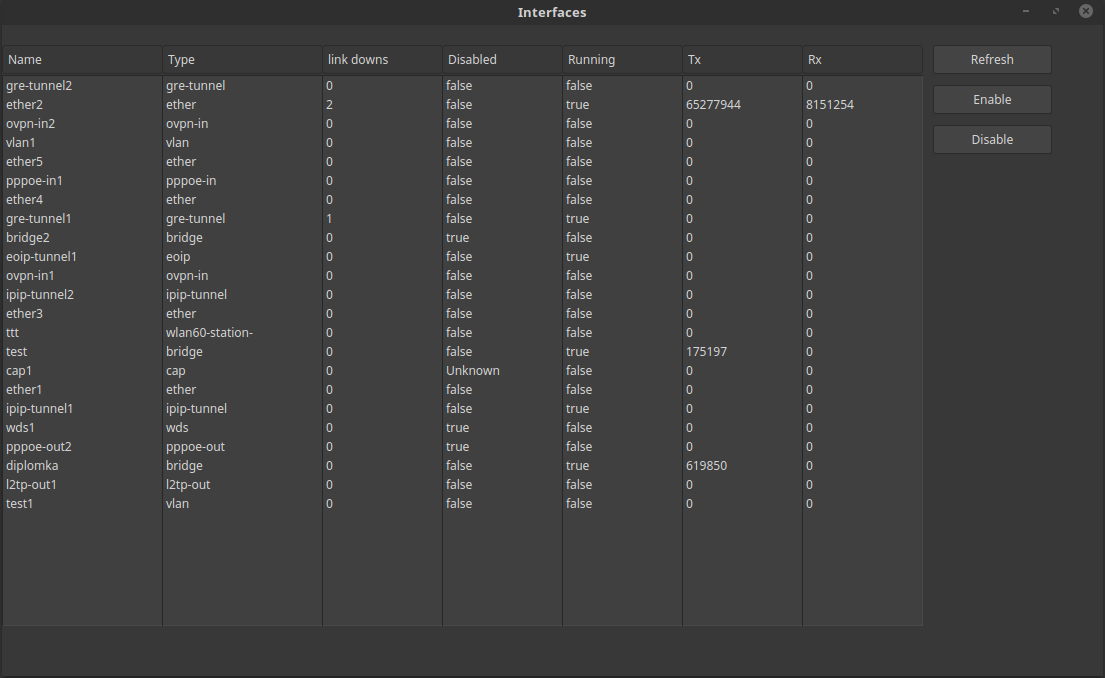
\includegraphics[scale=0.35]{../text/interfacesgui.png}
\caption{Okno interfaces}
\label{fig:interfacesgui}
\end{figure}
\begin{figure}[H]
\centering
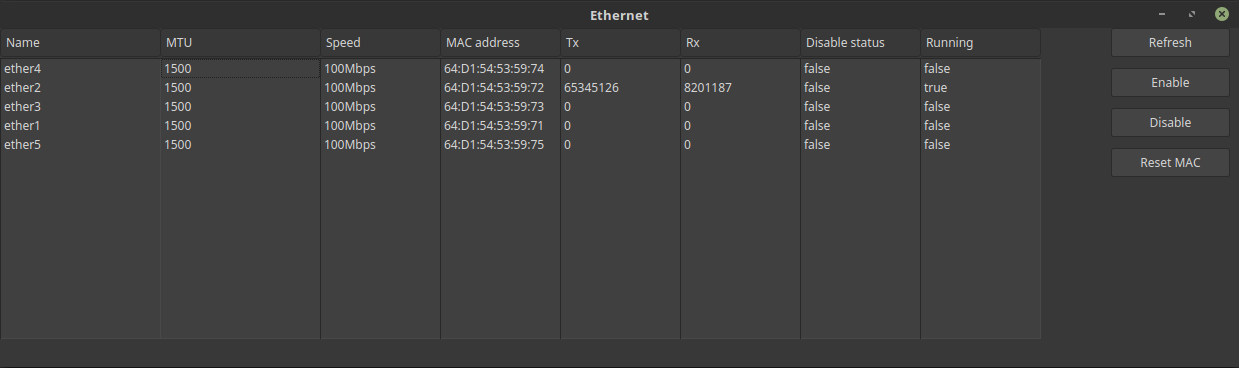
\includegraphics[scale=0.35]{../text/ethernet.png}
\caption{Okno ethernet}
\label{fig:ethernet}
\end{figure}
\begin{figure}[H]
\centering
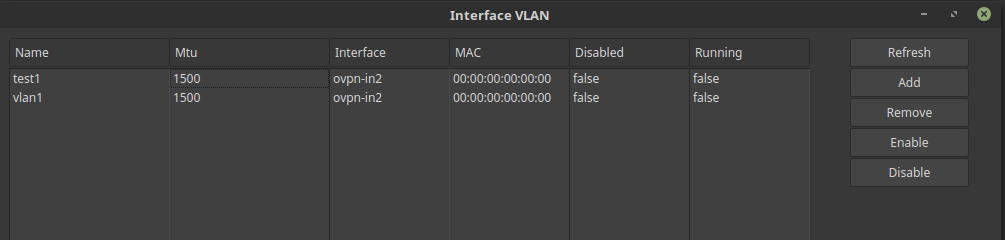
\includegraphics[scale=0.35]{../text/vlangui.png}
\caption{Okno VLAN}
\label{fig:vlangui}
\end{figure}
\begin{figure}[H]
\centering
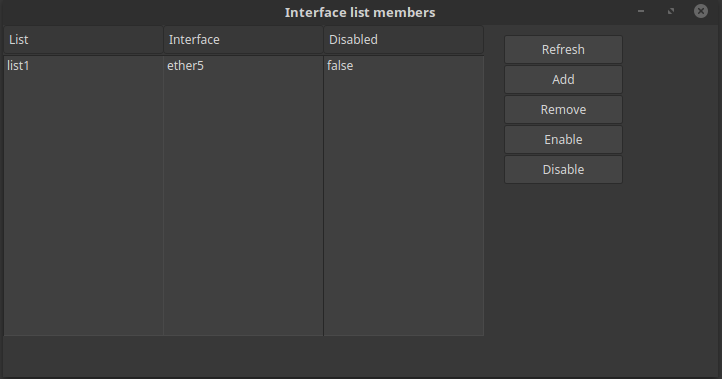
\includegraphics[scale=0.35]{../text/ifacelistmember.png}
\caption{Okno Interface list member}
\label{fig:interfacelistmembergui}
\end{figure}
\begin{figure}[H]
\centering
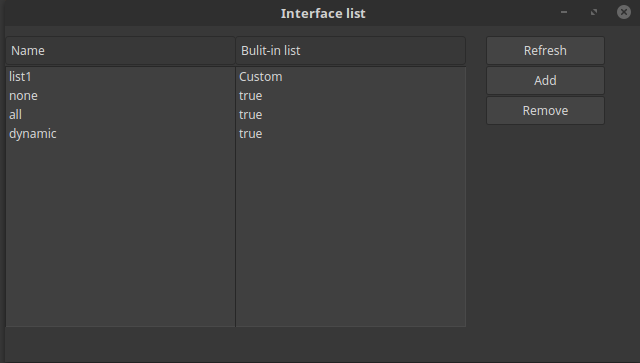
\includegraphics[scale=0.45]{../text/ifacelist.png}
\caption{Okno interface list}
\label{fig:interfacelistgui}
\end{figure}
V rámci aplikácie sa tu nachádzajú ďalších niekoľko okien, napr. IP, Maintenance, About, DHCP, Hostname, atď. Tieto časti aplikácie sú riešené rovnakým spôsobom ako to je v kapitole \ref{sec:gui}. Zoznam všetkých tlačítok sa nachádza v kapitole \ref{sec:buttons}.
\section{Testovanie aplikácie}
V rámci aplikácie bolo prevedené manuálne testovanie. Aplikácia bola tetsovaná na lokálnom mikrotiku, na ktorom bol nahratý a importovaný certifikát \textit{diplomlka.crt}. Tento certifikát bol následne použitý aj v službe API-SSL. V rámci testovania sú certifikáty nahraté aj v koreňovej zložke projektu aplikácie.\\
Ako prvé bolo otestované vyhľadávanie zariadení kliknutím na tlačítko "\textit{find devices}". Pre funkčnosť tohoto vyhľadávania je potreba vypnúť firewall, nakoľko linux so zapnutým firewallom zariadenia nevyhľadá.\\
Po vyhľadaní zariadení sa kliknutím na záznam IP adresy vloží do políčka "\textit{Address}". Štandardne tam je nastavené užívateľské meno \textit{admin}. Zadaním hesla a stalčením tlačítka \textit{OK} nastávajú situácie:
\begin{itemize}
\item úspešné prihlásenie otvorí okno s aplikáciou
\item neúspešné prihlásenie (užívateľské meno alebo heslo) vypíše výnimku do okna s textom "\textit{Could not login}"
\item posledná varianta je nepodpora API-SSL na zariadení, chyba certifikátu (overovanie) vyhodí výnimku do okna s textom "\textit{Could not open socket}"
\end{itemize}  
V rámci ďalšieho testovania nastávajú nasledujúce situácie:
\begin{itemize}
\item otestovanie otvorenia okien, okná sa otvárajú v hlavnom okne aplikácie, minimalizovaním hlavného okna aplikácie sa minimalizuje všetko, okná sú zoradené do kaskády
\item otestovanie tlačítok \textit{enable, disable} - tlačítkami sa otestuje vypnutie a zapnutie položky v aplikácii, niektoré položky nemožno vypnúť (napr. dynamické záznamy v ARP) a vyskočí oknos výnimkou "\textit{Could not talk to api}", čo v týchto prípadoch znamená, že prvok nie je možné vypnúť, obdobne to platí aj pre tlačítko \textit{Enable}, ďalej pri zapnutí a vypnutí položky sa v stĺpci disabled pri vypnutí nastaví paramter na True, v opačnom prípade na False
\item tlačítko remove - otestovanie tlačítka remove, ktoré odobere špecifický záznam na zariadení, obdobne ako pri zapnutí a vypnutí položky sa vyhodí rovnaká výnimka, po odobraní záznamu sa záznam odstráni aj z listu položiek a obnoví sa aktuálny zoznam 
\item otestovanie pridania položiek - otestuje sa pridanie položiek spôsobom, že sa ako prvé otvorí nové okno, kliknutím naň sa zobrazí  a pridajú sa konkrétne údaje, následne stalačením OK sa tento záznam pridá, platí to tiež pre okná s viac add tlačítkami, napr. pre firewall, logging, mangle, nat, v momente pridania záznamu  sa zoznam záznamov obnoví na aktuálny zoznam, pri výnimke, napr. zle zadanom údaji sa vyhodí výnimka s oknom "Could not talk to api"
\item testovanie Maintenance - tlačítkom sa otestujú funkcie - reštartovanie zariadenia, vypnutie zariadenia, upgrade zariadenia na main verziu, v prípade problému s pripojením sa vyhodí okno s výnimkou, zapnutie a vypnutie balíčkov, reset zariadenia, obnovenie zariadenia zo súboru
\item test Quit a About - tlačítkom about sa vyhodí okno s informáciou o softvéri, tlačítkom Quit sa ukončí celá aplikácia 
\end{itemize}
\chapter{Návod na inštaláciu a spustenie}
\section{Inštalácia na operačom systéme linux}
Najspoľahlivejšou cestou je nainštalovanie potrebných balíčkov v rámci pythonu na spustenie aplikácie. Linux v sebe štandardne zahrňuje python v oboch verziách, teda aj vo verzii 2 aj vo verzii 3, k posledným aktualizáciám linux mint vo verzii 3.6.5. \\
Tento návod bude popisovať spôsob nainštalovania potrebných súborov a modulov do pythonu, ako aj spôsob spustenia aplikácie. Návod bol písaný na distribúciu linuxu Linix Mint, toto vychádza z Ubuntu teda z Debianu. Pre CentOS sa použije buď \textit{dnf} alebo \textit{yum}, to platí aj pre  fedoru. Pre arch linux platí príkaz \textit{pacman} na nainštalovanie jednotlivých aplikácií. 
\subsection{Inštalácia pip a pip3}
Pre potrebu inštalovania modulov do pythonu je potreba doinštalovať inštalátor pip a pip3 (pre python vo verzii 3).
\begin{lstlisting}[language=bash, frame=single, caption=Nainštalovanie pip,captionpos=b, showstringspaces=false, basicstyle=\footnotesize]
sudo apt install python-pip
sudo apt install python3-pip
pip install --upgrade pip
pip3 install --upgrade pip
\end{lstlisting}
\subsection{Nainštalovanie knižnice tikapy}
\label{sec:tikapy}
Zadaním nasledujúceho príkazu v terminále sa nainštaluje knižnica tikapy, prte komunikáciu s mikrotikom, je použitá v backend časti aplikácie. Tikapy modul používa jazyk python 3. V prípade neúspechu je treba pridať parameter \textit{--user}.
\begin{lstlisting}[language=bash, frame=single, caption=Nainštalovanie tikapy,captionpos=b, showstringspaces=false, basicstyle=\footnotesize]
sudo apt install git
git clone https://github.com/vshn/tikapy
pip3 install tikapy
\end{lstlisting}
\subsection{Nainštalovanie pexpect}
Podobne ako v kapitole \ref{sec:tikapy}, je potreba doinštalovať modul pexpect, ktorý zahrňuje pxssh, pxtelnet, pxftp, ...
\begin{lstlisting}[language=bash, frame=single, caption=Nainštalovanie pexpect,captionpos=b, showstringspaces=false, basicstyle=\footnotesize]
pip install pexpect
pip3 install pexpect
\end{lstlisting}
\subsection{Inštalácia mactelnet}
Pre potrebu vyhľadávania zariadení v aplikácii je potreba nainštalovať mactelnet klienta. Toto sa vykoná vykonaním príkazu
\begin{lstlisting}[language=bash, frame=single, caption=Nainštalovanie mactelnet,captionpos=b, showstringspaces=false, basicstyle=\footnotesize]
sudo apt install mactelnet-client
\end{lstlisting}
\subsection{Nainštalovanie setuptools}
Pre možnosť používania modulov do pythonu je nutné nainštalovať setuptools, to sa prevedie príkazom
\begin{lstlisting}[language=bash, frame=single, caption=Nainštalovanie setuptools,captionpos=b, showstringspaces=false, basicstyle=\footnotesize]
pip install setuptools --user
pip3 install setuptools --user
\end{lstlisting}
\subsection{Inštalácia PyQT4}
Grafická časť aplikácie je napísaná v module jazyka python PyQT4. Na inštaláciu je potreba zadať príkaz
\begin{lstlisting}[language=bash, frame=single, caption=Nainštalovanie pyqt4,captionpos=b, showstringspaces=false, basicstyle=\footnotesize]
sudo apt install python-qt4 python-qt4-dev
sudo apt install python3-pyqt4
sudo apt install pyqt4-dev-tools
\end{lstlisting}
\subsection{Inštalácia QT4 designer}
Grafická časť aplikácie bola navrhnutá v programe \textit{QT4 designer}, pre jej spojazdnenie je potreba ju nainštalovať (jediné možné riešenie je len na operačnom systéme linux, na windows neexistuje inštalátor). Nainštaluje sa obdobne:
\begin{lstlisting}[language=bash, frame=single, caption=Nainštalovanie qt4 designera,captionpos=b, showstringspaces=false, basicstyle=\footnotesize]
sudo apt install python-qt4 qt4-designer
\end{lstlisting}
\subsection{Inštalácia paramiko}
Pre potreby fungovania aplikácie je potreba dpinštalovať modul paramiko. To sa prevedie príkazom
\begin{lstlisting}[language=bash, frame=single, caption=Inštalácia paramiko,captionpos=b, showstringspaces=false, basicstyle=\footnotesize]
pip install paramiko
pip3 install paramiko
\end{lstlisting}
\subsection{Spustenie aplikácie}
Aplikácia používa certifikáty uložené v projekte pod názvom \textit{diplomka1.crt} a kľúč k certifikátu pod názvom \textit{diplomka1.key}. Toto je pre spojenie s mikrotikom cez API-SSL. Pre spustenie aplikácie je potreba navigácie do koreňovej zložky, kde sa nachádza súbor \textit{loginGui.py}, tento súbor je spúšťací súbor na spustenie napísanej GUI aplikácie. Následne sa program spustí nasledovne:
\begin{lstlisting}[language=bash, frame=single, caption=Spustenie aplikácie,captionpos=b, showstringspaces=false, basicstyle=\footnotesize]
adrian@~/PycharmProjects/diplomkap3 $ python3 loginGui.py
\end{lstlisting}
Po úspešnom spustení by sa malo otvoriť prihlasovacie okno, kde po jeho inicializácii sa stlačením tlačítka na vyhľadanie zariadení cez tlačítko \textit{FInd devices}, toto trvá 1 minútu kým program mactelnet nájde najbližšie zariadenia, štandardné prihlasovacie užívateľské meno je \textit{admin}, po kliknutí na IP adresu sa doplní do textového poľa address. Následne sa zadá heslo a stlačí sa tlačítko OK. 
\section{Návod na inštaláciu na operačnom systéme Windows}
Aplikácia je napísaná vo verzii PyQt 4, ktorá existuje pre Windows do verzii pythonu 3.3, pre využitie vyšších verzií pythonu je nutné používať PyQt 5. Inštalácia je nasledujúca.
\subsection{Inštalácia Python 3.3}
Stiahnutie a inštalácia \textit{.exe} inštalátoru z nasledujúceho \href{http://www.python.org/ftp/python/3.3.5/python-3.3.5.amd64.msi}{odkazu} pre 64-bitovú platformu a pre 32-bitovú platformu z \href{http://www.python.org/ftp/python/3.3.5/python-3.3.5.msi}{odkazu}. Následne je potreba nastaviť systémovú premennú, aby sa mohol volať príkaz \textit{python3}, prípadne \textit{python} sa toto nastaví v rámci inštalátoru. 
Možné nastavenie systémovej premennej je vidieť na obrázku \ref{fig:premenna}.
\begin{figure}[H]
\centering
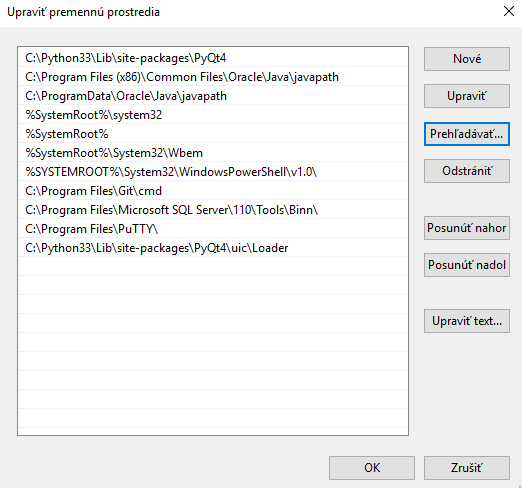
\includegraphics[scale=0.6]{../text/premenna.png}
\caption{Nastavenie systémovej premennej na windowse}
\label{fig:premenna}
\end{figure}
\subsection{Inštalácia pip}
Python inštalátor nezahrňuje pip prípadne pip3 a preto je nutné ho doinštalovať nasledovne:
\begin{enumerate}
\item stiahnutie súboru \href{https://bootstrap.pypa.io/get-pip.py}{\textit{get-pip.py}} do zložky kde je python, štandardne na disku C v zložke Python33. 
\item nainštalovanie pip pomocou príkazu: \textit{python.exe get-pip.py}. Po úspešnej inštalácii sa tu objaví zložka \textit{Scripts}, \textbf{zložka musí obshaovať súbory pip a pip3}.
\end{enumerate}
\subsection{Inštalácia modulov}
Doinštalovanie modulov tikapy, pexpect, paramiko, pypi nasledovne. Cez prieskumník sa dostaneme do zložky Scripts, kde pomocou pravého tlačítka myši a tlačítka SHIFT (ľavý) sa otvorí ponuka otvoriť cez powershell. Následne sa zadajú príkazy:
\begin{itemize}
\item \textit{.\textbackslash pip3 install tikapy} 
\item \textit{.\textbackslash pip install tikapy}
\item \textit{.\textbackslash pip3 install pipy}
\item \textit{.\textbackslash pip install pipy}
\item \textit{.\textbackslash pip3 install paramiko}
\item \textit{.\textbackslash pip install paramiko} 
\item \textit{.\textbackslash pip3 install pexpect}
\item \textit{.\textbackslash pip install pexpect}
\item \textit{.\textbackslash pip3 install setuptools}
\item \textit{.\textbackslash pip install setuptools}   
\end{itemize}
\subsection{Inštalácia PyQt4}
Pre nainštalovanie PyQt 4 na Windowse, je potreba stiahnuť \textit{.exe} inštalátor a nainštalovať ho do zložky, kde sa nachádza python, čo je štandardne \textit{C:\textbackslash python33}. Tu sa následne vytvoria všetky potrebné súbory na spustenie GUI aplikácie.
\subsection{Spustenie aplikácie}
Pre spustenie aplikácie je potreba pristupovať absolútnymi cestami. To je, pre spustenie aplikácie je nutné sa prenavigovať do zložky s projektom, ktorý je možný stiahnúť z priloženého DVD. Následne spustiť príkaz, napr. projekt mám uložený v adresáry E:\textbackslash diplomka. Potom príkaz bude vypadať \textit{C:\textbackslash python33\textbackslash python.exe loginGui.py}.
\subsection{Možné problémy na windowse}
Niektoré verzie Windows nepodporujú PyQt 4, preto môže vzniknúť situácia že sa aplikácia nespustí. Dôvodom môže byť, že nedokáže nájsť knižnicu \textit{uic}, ktorá je súčasťou PyQt 4. Pokiaľ to nepôjde sú tu dva scenáre:
\begin{itemize}
\item Scenár 1: Nastavenie systémovej premennej podobne ako na obrázku \ref{fig:premenna} pre uic, ktoré je v zložke kde sa nachádza python
\item Scenár 2: Preportovanie aplikácie do verzie PyQt 5
\end{itemize}  

